\documentclass[../main.tex]{subfiles}

\begin{document}

\chapter{Drivers of Antarctic Ice}
\label{chap:environmenal_drivers}


% The variable which we found had the largest impact on the behaviour of ice in Antarctica is temperature. This follows naturally from the basic thermodynamics of phase change. As the temperature increases we see lower concentrations of sea ice, and as the temperature increases we see lower concentrations of sea ice. The extent of this relationship will be explored in detail in this chapter. We will first look at the relationship through density plots \textcolor{red}{Check name of plots}. Before calculating correlations and looking at the similarities and differences of the two different variables.

% For the purpose of this chapter, when we use temperature we will use \gls{skt} as discussed before \textcolor{red}{Write up different temperatures.}

% In chapter \ref{chap:temp_and_ice}, we found that temperature is significant for our understanding of the trends in Antarctic \gls{sic} over the last 40 years. However we found that the relationship between temperature and land ice is not as strong. To understand this we will have to do some more calculations.

% We want to consider a range of variables which could be impacting land ice in Antarctica. We will include temperature again for completeness. Wind speed is linked to atmospheric circulations which move clouds and thermal energy around the continent. Cloud cover has also been linked to behaviours in the land ice. \todo{add appropriate citations here}. 

Now we understand something of how ice in Antarctica has behaved over the last 40 years both over land and sea, we want to understand what dives the trends and variability which we have observed in chapter \ref{chap:ice_behaviour}. This will be the main focus of this chapter. First, we will briefly summarise the variables discussed in literature which we might expect to impact the behaviour of Antarctic ice. We will briefly revisit the technicalities of using the different datasets we have for different variables and the implications this has for our analysis. Then we will explore briefly some observational statistics for the different variables we are interested in. Plotting trends and mean timer-series for each variable and discussing any immediately apparent relationships between the different variables. We will carry out regression analysis, comparing each environmental variable with Antarctic ice, and finally we will do multi-regression analysis to complete our statistical analysis of what drives Antarctic Ice.


\section{Variables discussed in literature}
\begin{figure}[hbt!]
    \centering
    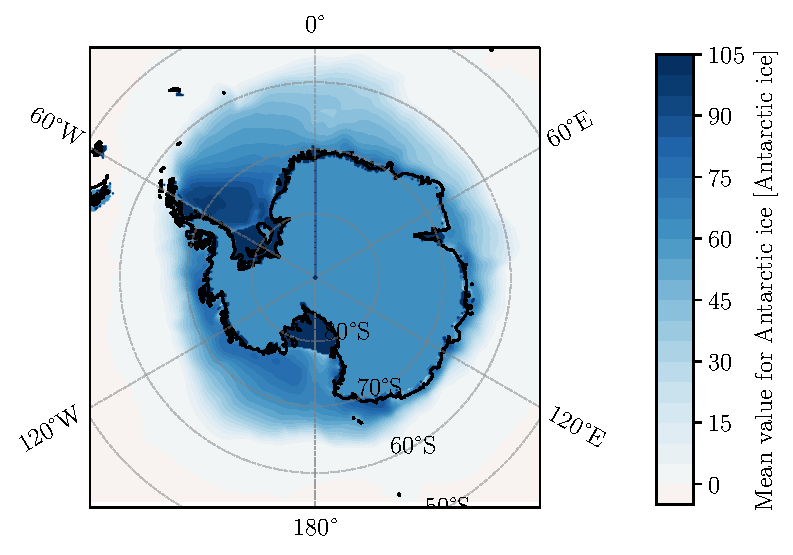
\includegraphics{images/T2/mean_spatial/hres/ICE}
    \caption{Caption}
    \label{fig:mean_spatial_LIC}
\end{figure}

\section{Trends in Variables}

\section{Regression Analysis}

\section{Multiple Regression Analysis}





\end{document}